% Chapter 5

\chapter{Implementation} % Main chapter title

\label{Chapter5} % For referencing the chapter elsewhere, use \ref{Chapter5} 

\lhead{Chapter 5. \emph{Algorithms}} % This is for the header on each page - perhaps a shortened title

%----------------------------------------------------------------------------------------

\section{Correct Sequences}
Suppose the following are a run sequence and a frequent sequence.
We need to find out if the frequent sequence is present in a run sequence. But how do we decide of all the combinations possible which ones to select?

\subsection{Run Sequence}
Run Sequences are provided as input in a JSON file. They denote the order of the  method invocations of the acceptance test.\\
\begin{tabular}{l|llllllllllllllll}
run sequence& 1 &4 &5 &4 &36 &84 &1 &3 &4 &5 &8 &17 &99 &8 &32 &9\\
\hline
 counters&0 &1 &2 &3 &4  &5  &6  &7  &8  &9 &10 &11 &12 &13 &14 &15 \\
\end{tabular}

\subsection{Frequent Sequence}
Frequent Sequence is one of the many output sequences that BIDE provide in frequent.dat file.
It is closed and maximal
Suppose one of the frequent sequence is 1 4 5

\subsection{Analysis}
So let's see which of the few possible sequences are correct or useful for us.\\
As there can be repetetive functions for the same run sequence, we will uniquely identify the method with respect to the counter number.

\checkmark\tab 0 1 2\\
\tab This is a straightforward consecutive sequence and is valid.

\checkmark \tab0 3 9\\
\tab This is also a valid sequence as 1 4 5 appear in order though they are not consecutive.

{\large{X}}\tab 6 3 9\\
\tab This will not be considered valid because though the counters suggest 1 4 5 but they are not in order and with respect to integration testing run sequences are ordered so in other words we donot have the state of functions in that order and thus we are not interested in these types of sequences as they do not occur.

\section{Block Structure}
The Fig.\ref{algo} explains the basic blocks of the project.\\
They consist of various sub functions and/or helping functions that we will see in the detailed explanation.

\begin{figure}[h]
\centering
 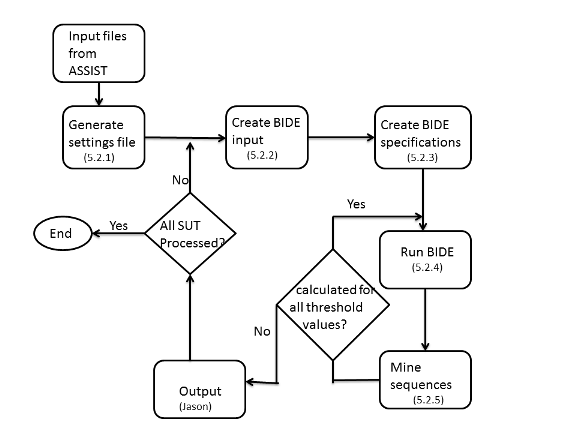
\includegraphics{algo}
\caption{Project Implementation.}
\label{algo}
\end{figure}

\subsection{Generate Settings File}
Before starting the program one needs to set the values of Settings.java file.\\
This is a static class which holds various values which are user inputs and which remain constant throughout the program.\\
They are:
\begin{itemize}
\item basePath : The folder where all the SUT folders reside
\item subjectAppName : The name of the SUT (to be appended to basePath)
\item thresholdValues : The array which stores all the threshold values for BIDE for which the SUT will be tested and results will be stored under the folder basePath/subjectAppName/thresholdValue.
\item methodMapFile : File name format for the input JSON file which maps each method with its name and class name to a unique number
\item sequenceMapFile : File name format for the Run Sequences in JSON file.
\end{itemize}
\tab and similar BIDE related data \dots

\subsection{Create BIDE Input}
This module takes care of converting the Run Sequences in input files from the JSON format to the textual-dataset (format required by the BIDE), explained in the Tools Section.\\
For each Run Sequence the data is extracted from JSON packets and stored in an BIDE input file.

\subsection{Create BIDE Specification}
While parsing the run sequences, ststistics required by the specification file format of BIDE are calculated.
They are:
\begin{itemize}
\item Number of Unique Items(Total number of methods, obtained from methodMap)
\item Number of Sequences(Total number of Run Sequences in input file)
\item Maximum length of sequences(Keeping a track while parsing from JSON)
\item Average length of sequence(Keeping a track while parsing)
\end{itemize}

\subsection{Run BIDE}
This module is called for each value of threshold mentioned in the Settings file.\\
An Operating System Process is borrowed and the BIDE executable is run on a Runtime Data Structure each time the module is called. There are two types of executables, one is with output on console and one is without output. The one with output can be used for logging purposes.

\subsection{Mine Sequences}
This module is the heart of the project. Most of the computative things happen in this module. There are various helper and subfunctions in this module. We will discuss them in detail in the following subsections.

\emph{Global Parameters for the module} : \{JSONObject, JSONArray, iterator, JSONParser\}

Let us see a combined pseudocde for an overview:
\subsubsection{getOccurence()}
\tab\emph{parameters} : Frequent Sequence\\
\tab\emph{return value} : All Subsequences from all the Run Sequences\\
\tab\emph{body} : Iterates over all Run Sequences and calls a helper function getSubSequences()

\subsubsection{getSubSequence()}
\tab\emph{parameters} : Frequent Sequence, Run Sequence, Counters of Run Sequence\\
\tab\emph{return value} : All the Subsequences of a particular Run Sequence\\
\tab\emph{body} : Calls getIndividualSet()\\
\tab\tab\tab 		        do\{\\
\tab\tab\tab\tab				add another item and create all possible combinations\\
\tab\tab\tab\tab				check if combination is a correct one\\
\tab\tab\tab\tab				reject the incorrect combination\\
\tab\tab\tab			\}\\
\tab\tab\tab			while(all items of frequent set covered)\\
This solution is inspired from the classic computer NP-Hard problem of Longest Common Subsequence\cite{lcs}.

			
\subsubsection{getIndividualSet()}
\tab\emph{parameters} : Frequent Sequence, Run Sequence, Counters of Run Sequence\\
\tab\emph{return value} : Sets, for each item in the frequent set, consisting of all the occurences in run sequence\\
\tab\emph{body} : for(each item in frequent set)\{\\
\tab\tab\tab 			for(each item in Run Sequence)\{\\
\tab\tab\tab\tab			if(items match)\{\\
\tab\tab\tab\tab\tab			add counter in the return list\\
\tab\tab\tab\tab 			\}\\
\tab\tab\tab 			\}\\
\tab\tab 		\}\\
				